\documentclass[twocolumn,a4j]{jsarticle}
\setlength{\topmargin}{-20.4cm}
\setlength{\oddsidemargin}{-10.4mm}
\setlength{\evensidemargin}{-10.4mm}
\setlength{\textwidth}{18cm}
\setlength{\textheight}{26cm}

\usepackage[top=15truemm,bottom=25truemm,left=15truemm,right=15truemm]{geometry}
\usepackage[latin1]{inputenc}
\usepackage{amsmath}
\usepackage{amsfonts}
\usepackage{amssymb}
\usepackage[dvipdfmx]{graphicx}
\usepackage[dvipdfmx]{color}
\usepackage{listings}
\usepackage{listings,jvlisting}
\usepackage{geometry}
\usepackage{framed}
\usepackage{color}
\usepackage[dvipdfmx]{hyperref}
\usepackage{ascmac}
\usepackage{enumerate}
\usepackage{tabularx}
\usepackage{cancel}
\usepackage{scalefnt}

\renewcommand{\figurename}{Fig.}
\renewcommand{\tablename}{Table }

\lstset{
basicstyle={\ttfamily},
identifierstyle={\small},
commentstyle={\smallitshape},
keywordstyle={\small\bfseries},
ndkeywordstyle={\small},
stringstyle={\small\ttfamily},
frame={tb},
breaklines=true,
columns=[l]{fullflexible},
xrightmargin=0zw,
xleftmargin=3zw,
numberstyle={\scriptsize},
stepnumber=1,
numbersep=1zw,
lineskip=-0.5ex
}

\makeatletter
\def\@maketitle
{
\begin{center}
{\LARGE \@title \par}
\end{center}
\begin{flushright}
{\large 報告書 NO.08 - 2\quad\@date\quad\@author}
\end{flushright}
\par\vskip 1.5em
}
\makeatother

\setcounter{tocdepth}{3}

\author{来代 勝胤}
\title{令和3年度 12月 第3週 報告書}
\date{2021/12/17}

\begin{document}
\columnseprule=0.1mm

\maketitle
\section*{報告内容}
\begin{enumerate}[1.]
    \item 進捗状況
    \item 模擬実験結果
\end{enumerate}

\section{進捗状況}
今週は,引き続き模擬実験を行った。
また,その実験結果のデータ処理を行った。

\section{模擬実験結果}

\begin{table}[htbp]
    \begin{center}
        \caption{Summary of root sum square value}
        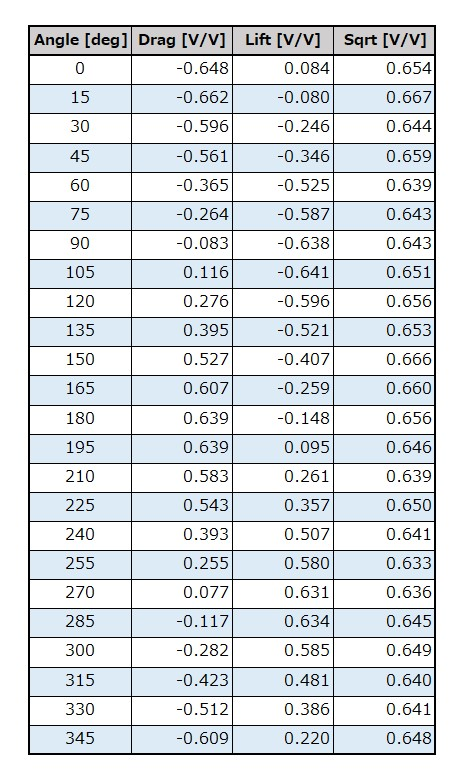
\includegraphics[width=90mm]{../images/table_1.jpg}
    \end{center}
\end{table}

\begin{figure}[htbp]
    \footnotesize
    \begin{center}
        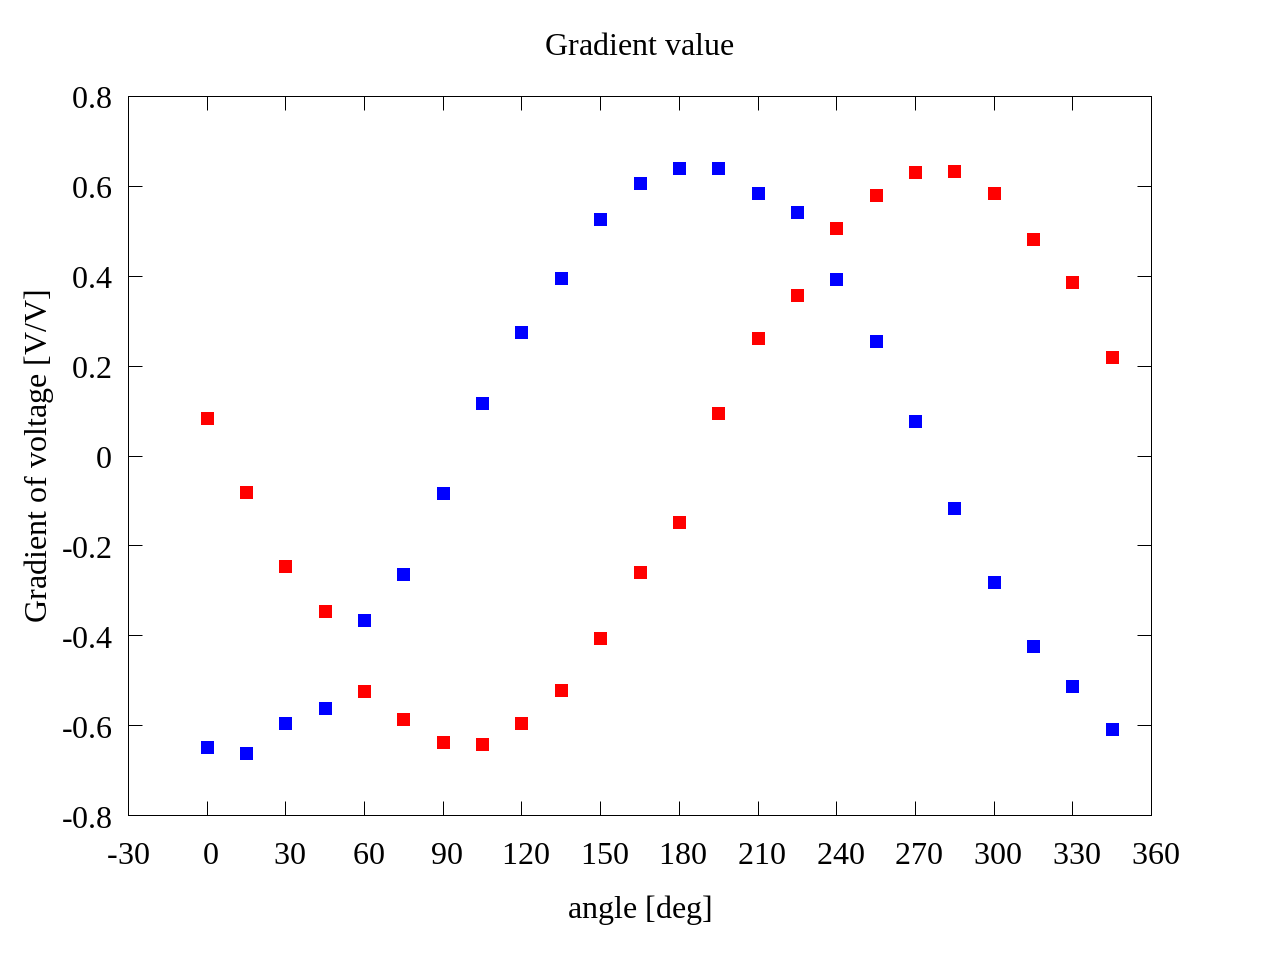
\includegraphics[width=85mm]{../images/summary/summary_1.png}
        \caption{Summary of gradient value}
        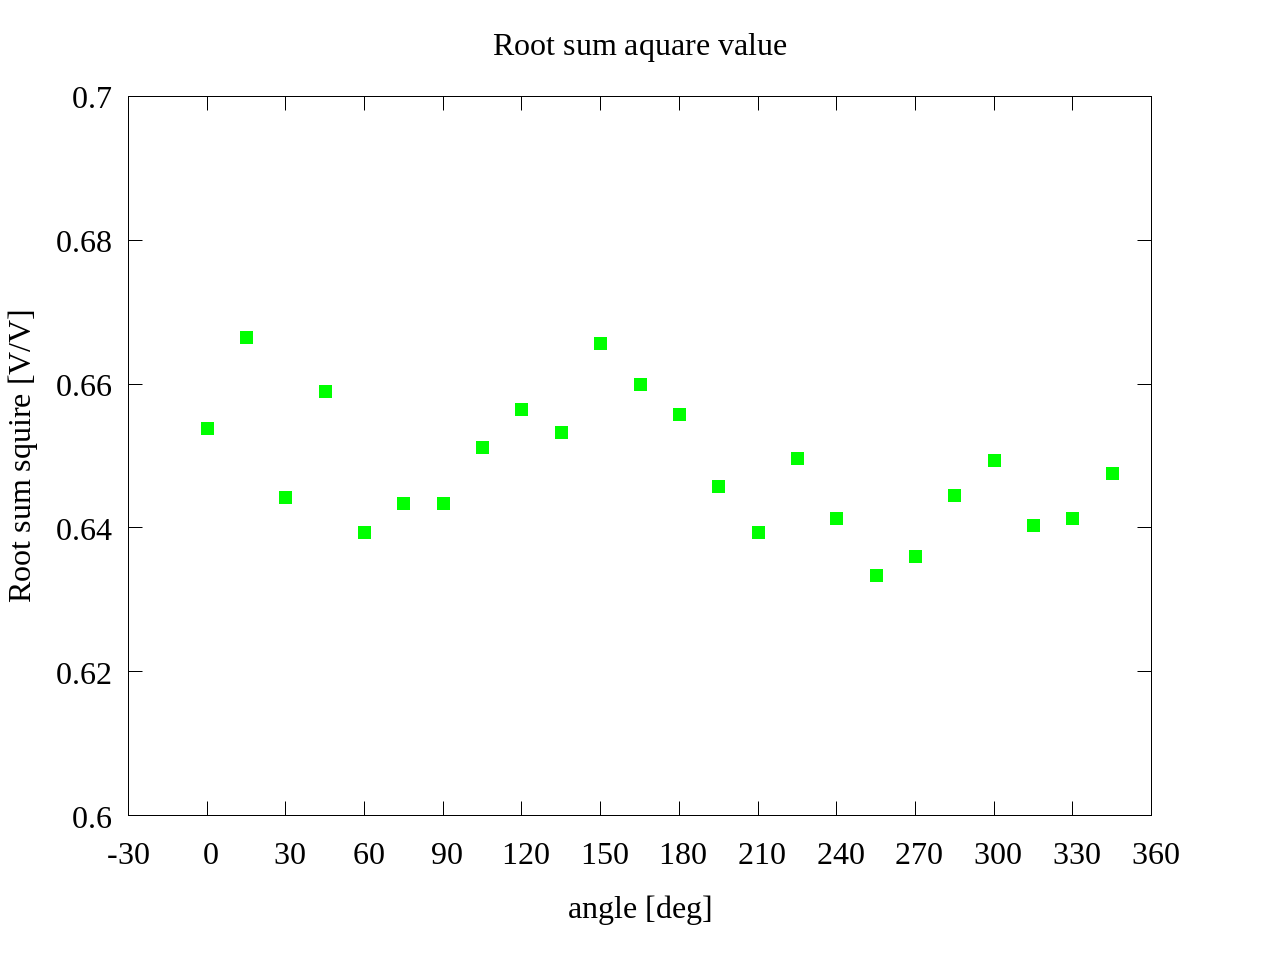
\includegraphics[width=85mm]{../images/summary/summary_2.png}
        \caption{Summary of root sum square value}
    \end{center}
\end{figure}

\begin{figure}[htbp]
    \footnotesize
    \begin{center}
        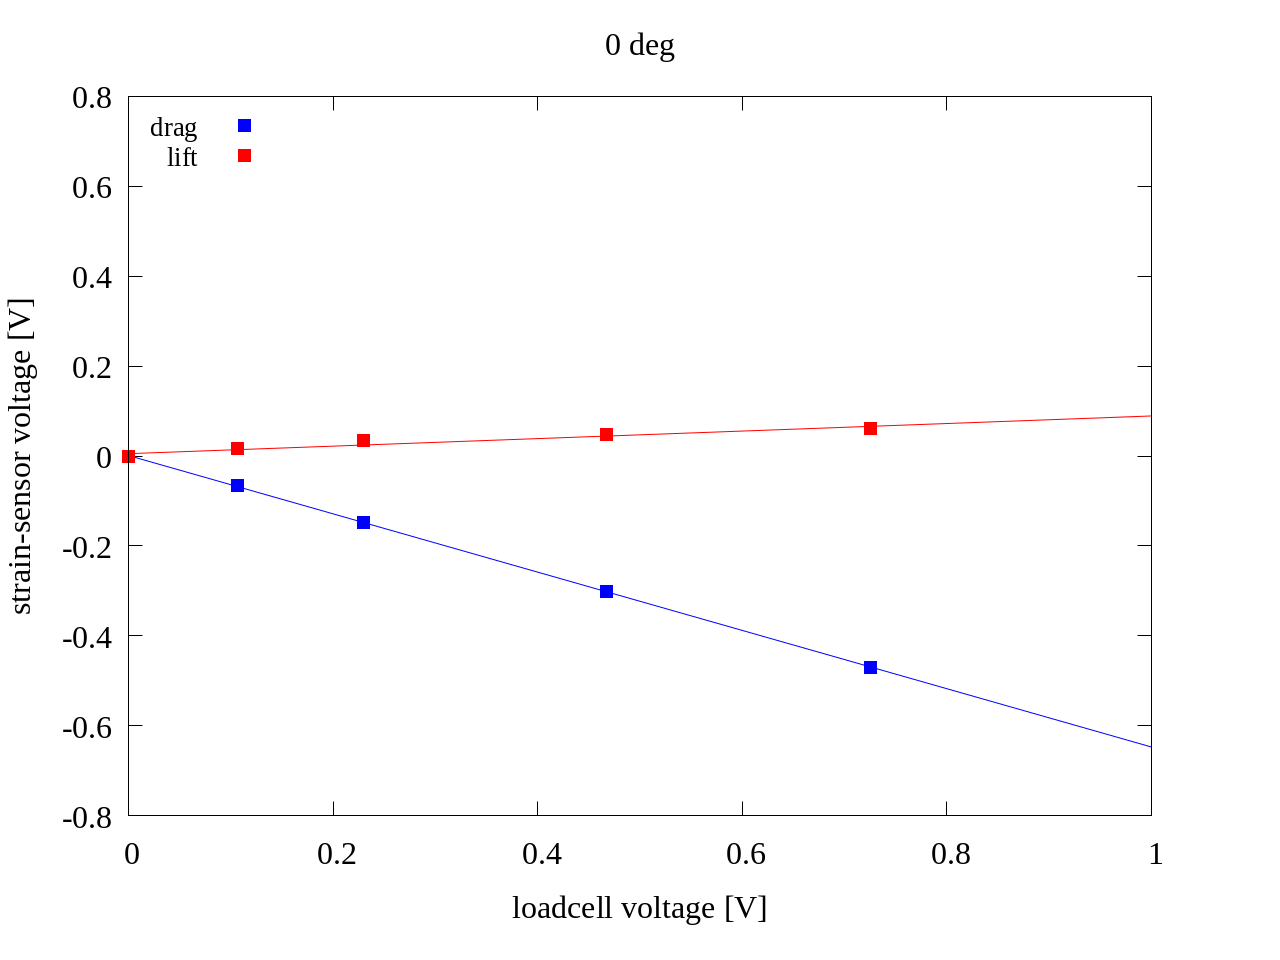
\includegraphics[width=78mm]{../images/linear/0_linear.png}
        \caption{Result of 0 deg}
        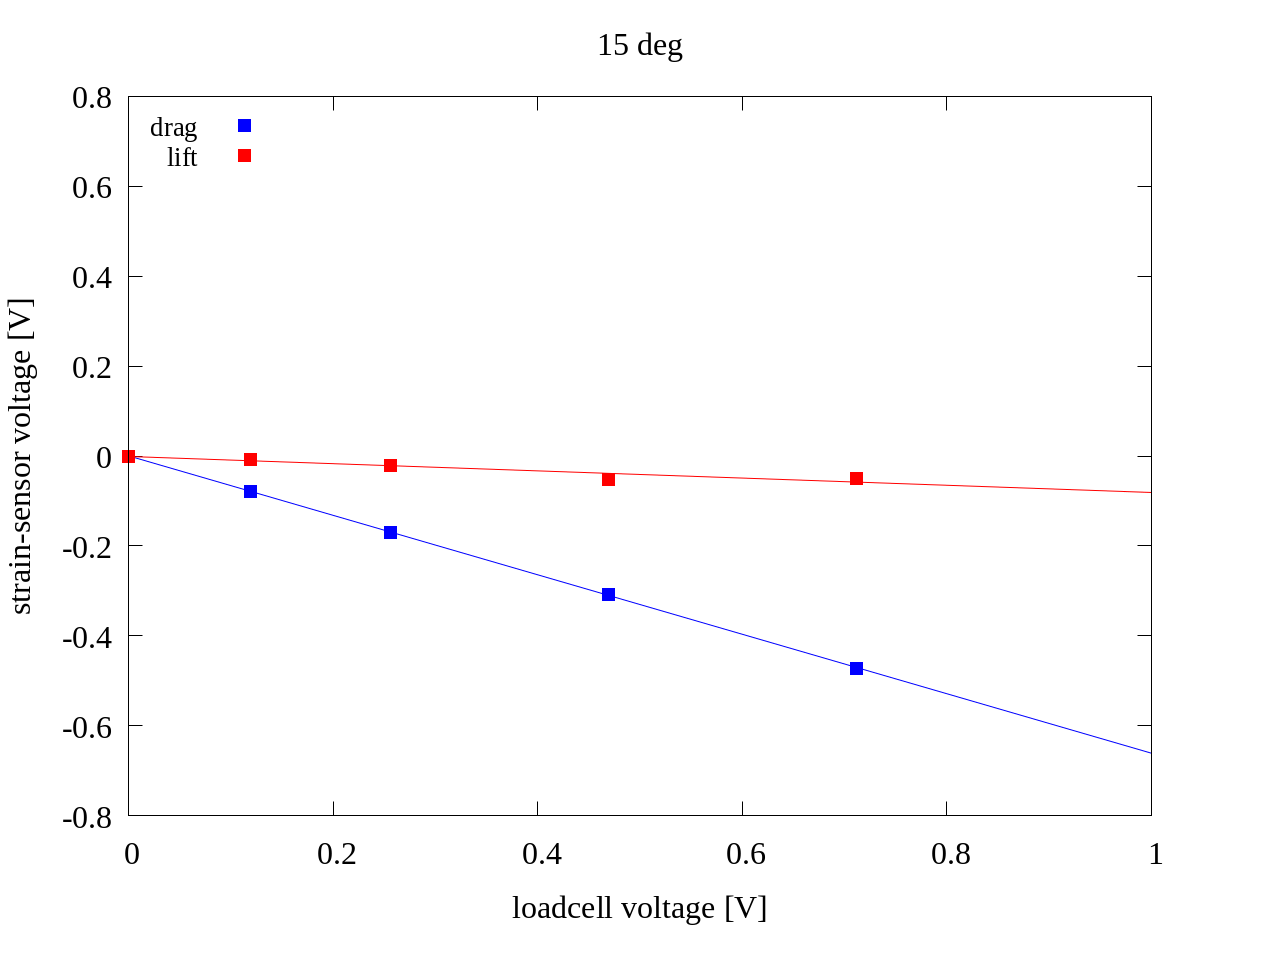
\includegraphics[width=78mm]{../images/linear/15_linear.png}
        \caption{Result of 15 deg}
        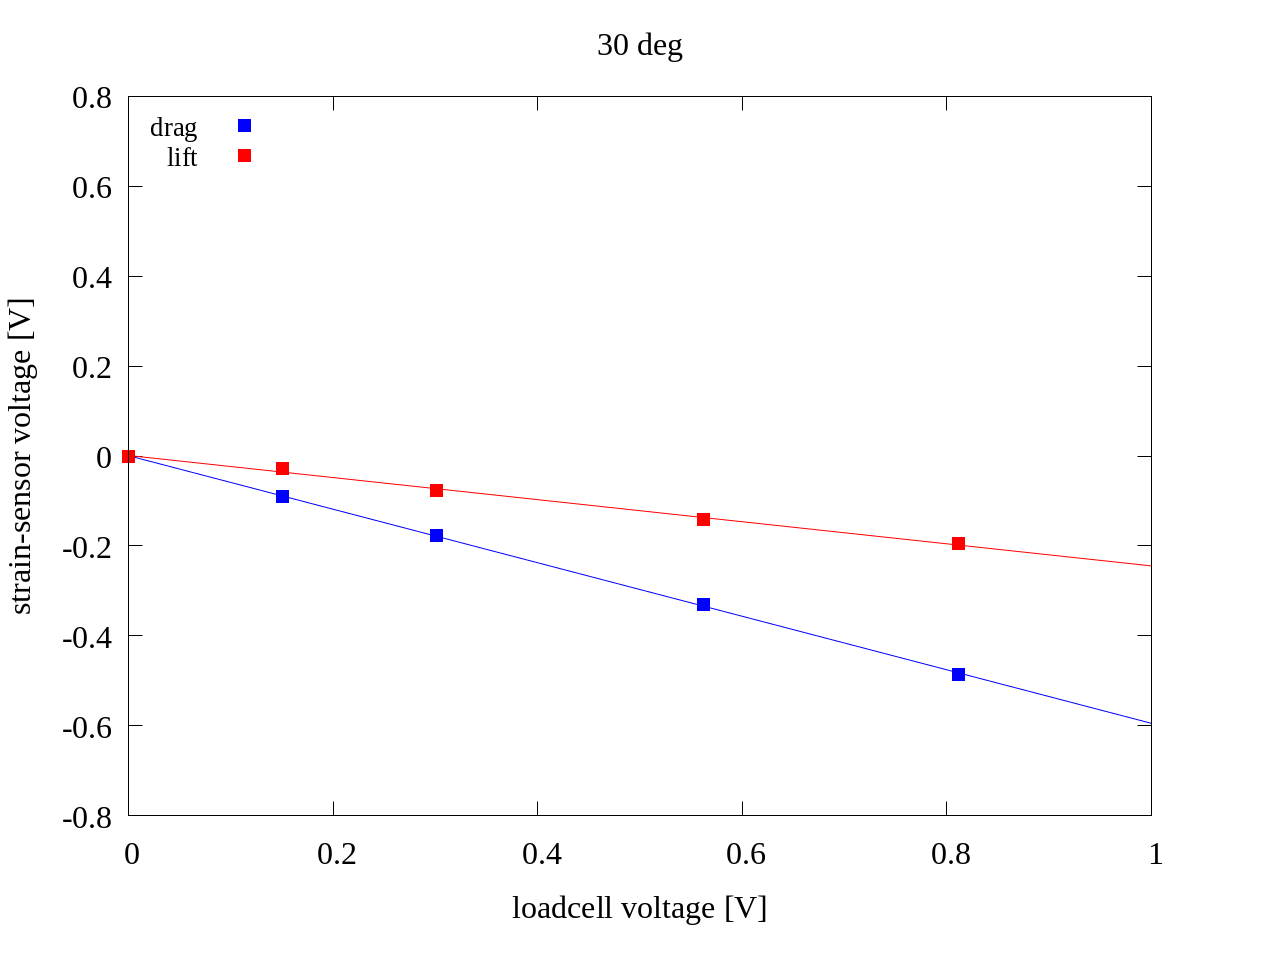
\includegraphics[width=78mm]{../images/linear/30_linear.png}
        \caption{Result of 30 deg}
        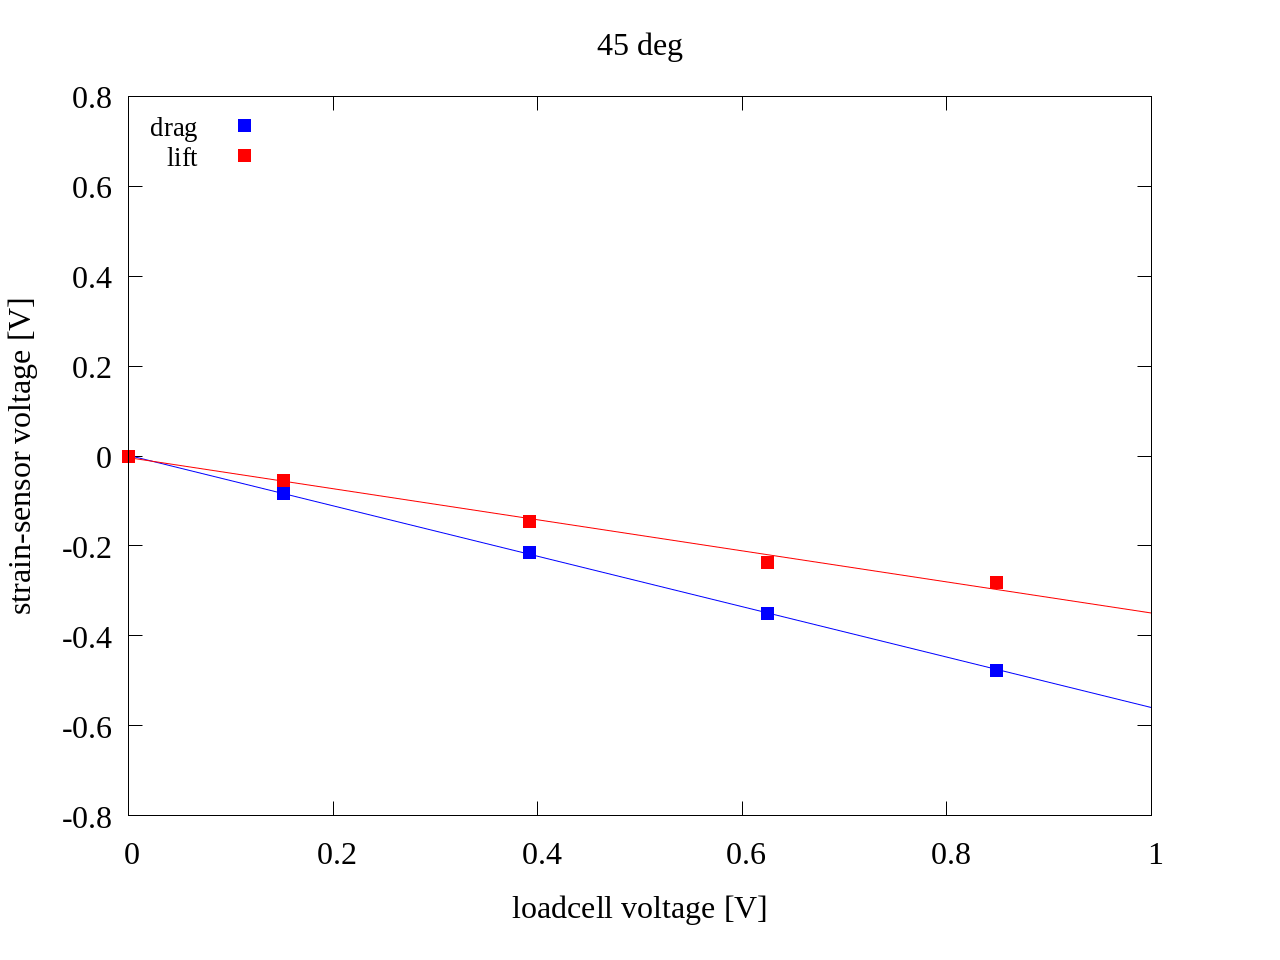
\includegraphics[width=78mm]{../images/linear/45_linear.png}
        \caption{Result of 45 deg}
    \end{center}
\end{figure}

\par
\newpage

\begin{figure}[htbp]
    \footnotesize
    \begin{center}
        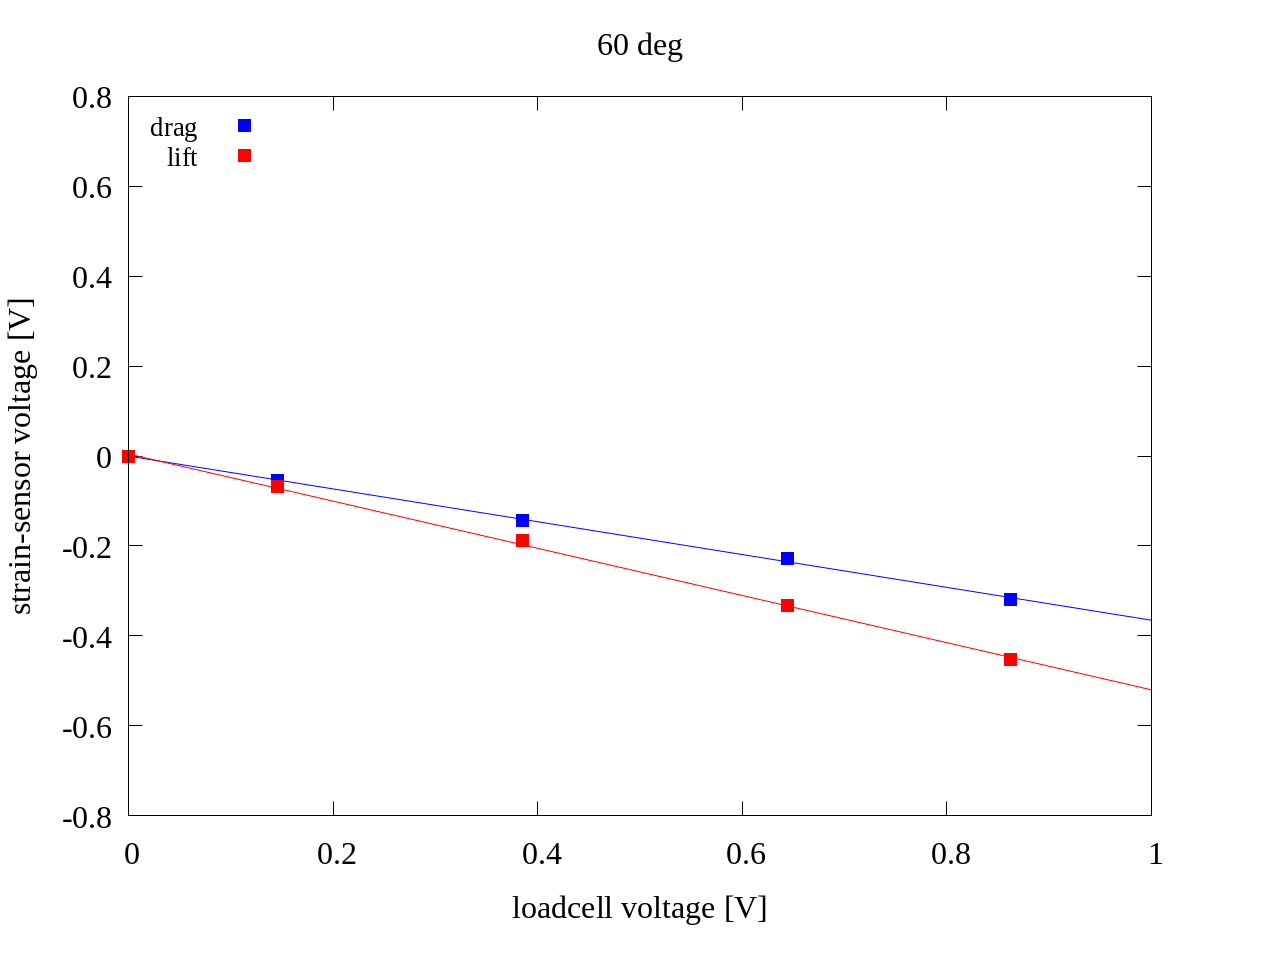
\includegraphics[width=78mm]{../images/linear/60_linear.png}
        \caption{Result of 60 deg}
        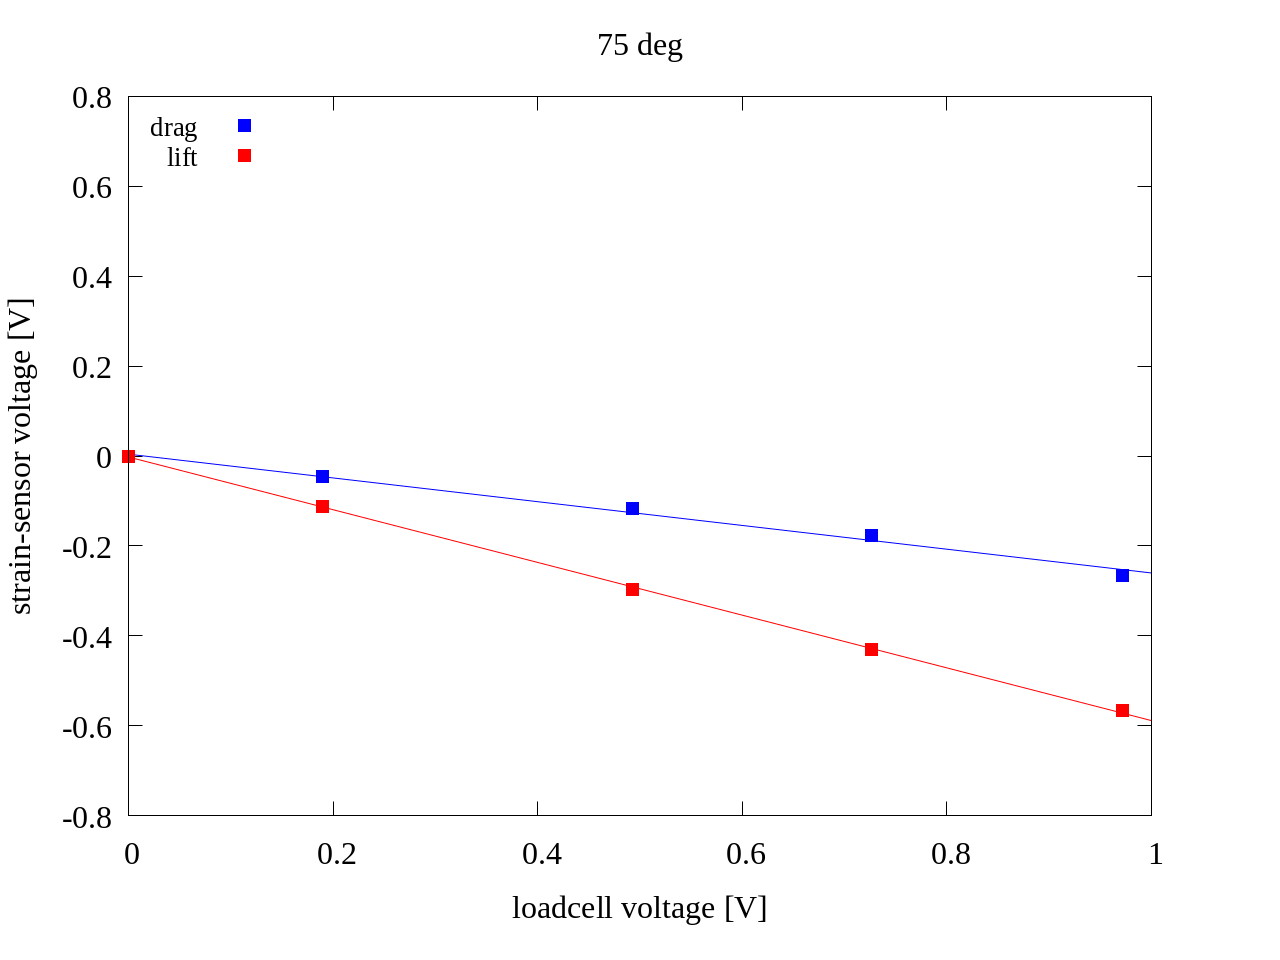
\includegraphics[width=78mm]{../images/linear/75_linear.png}
        \caption{Result of 75 deg}
        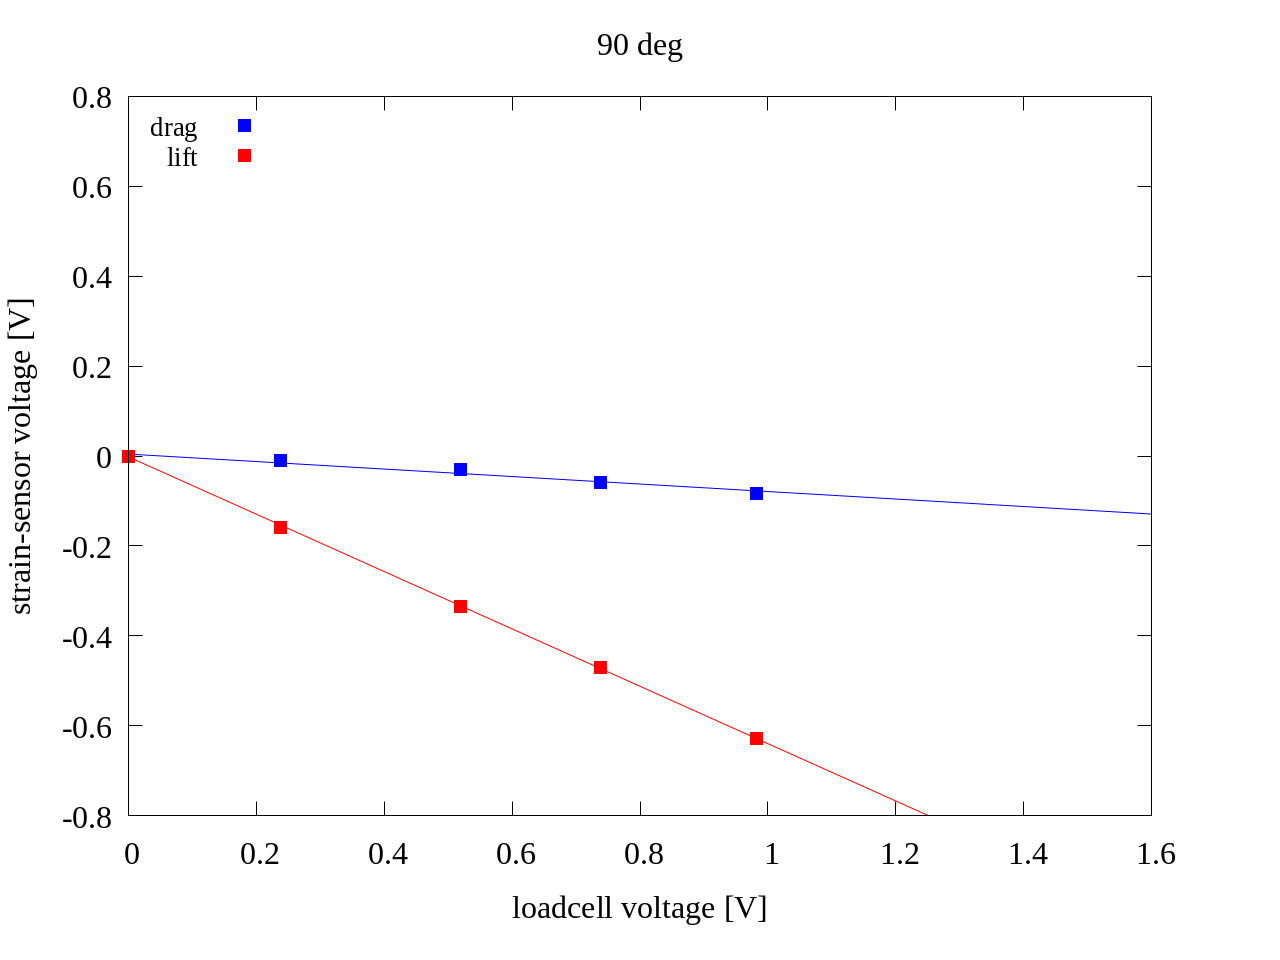
\includegraphics[width=78mm]{../images/linear/90_linear.png}
        \caption{Result of 90 deg}
        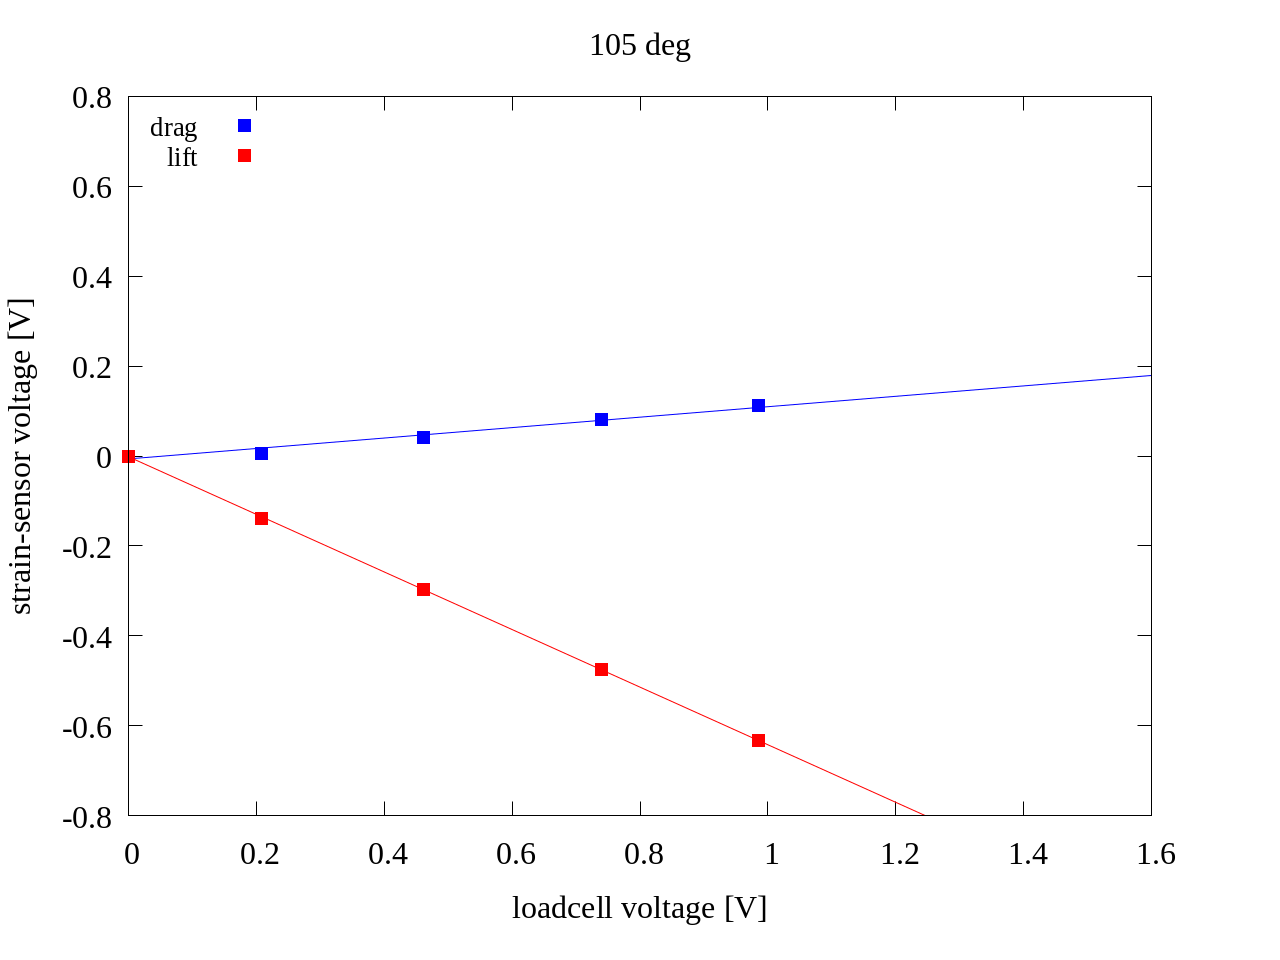
\includegraphics[width=78mm]{../images/linear/105_linear.png}
        \caption{Result of 105 deg}
    \end{center}
\end{figure}

\par
\newpage

\begin{figure}[htbp]
    \footnotesize
    \begin{center}
        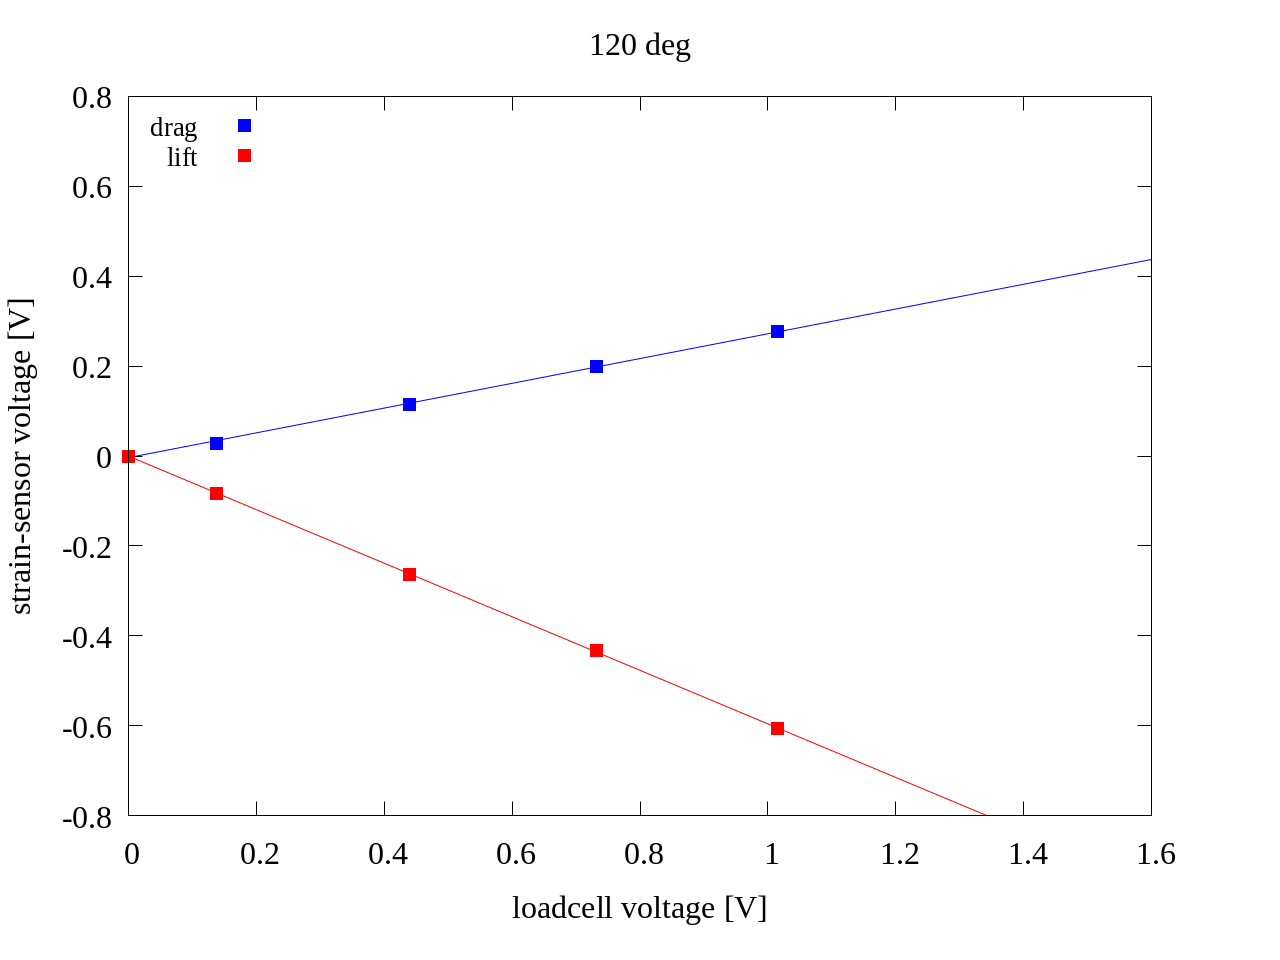
\includegraphics[width=78mm]{../images/linear/120_linear.png}
        \caption{Result of 120 deg}
        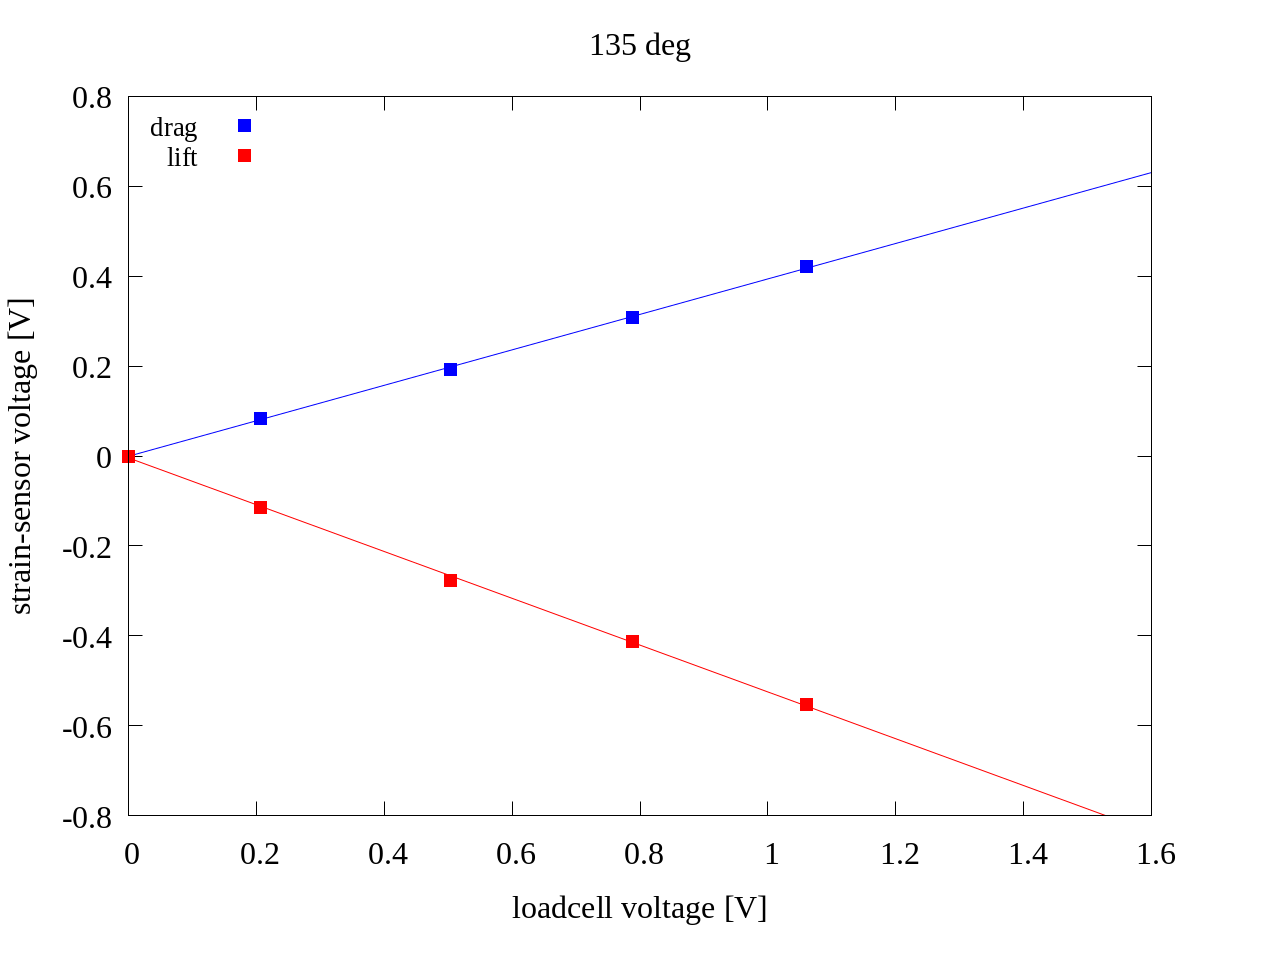
\includegraphics[width=78mm]{../images/linear/135_linear.png}
        \caption{Result of 135 deg}
        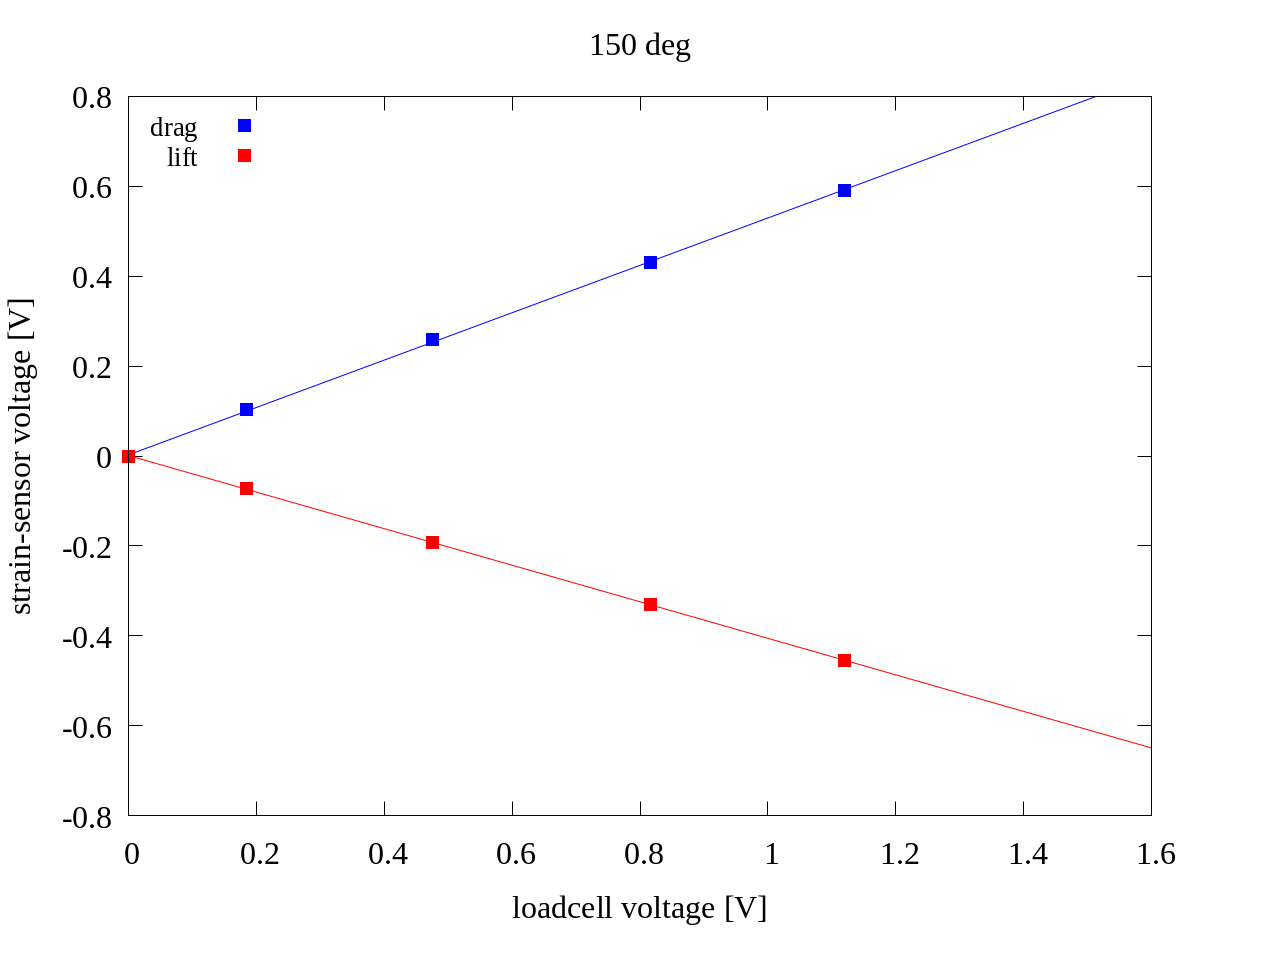
\includegraphics[width=78mm]{../images/linear/150_linear.png}
        \caption{Result of 150 deg}
        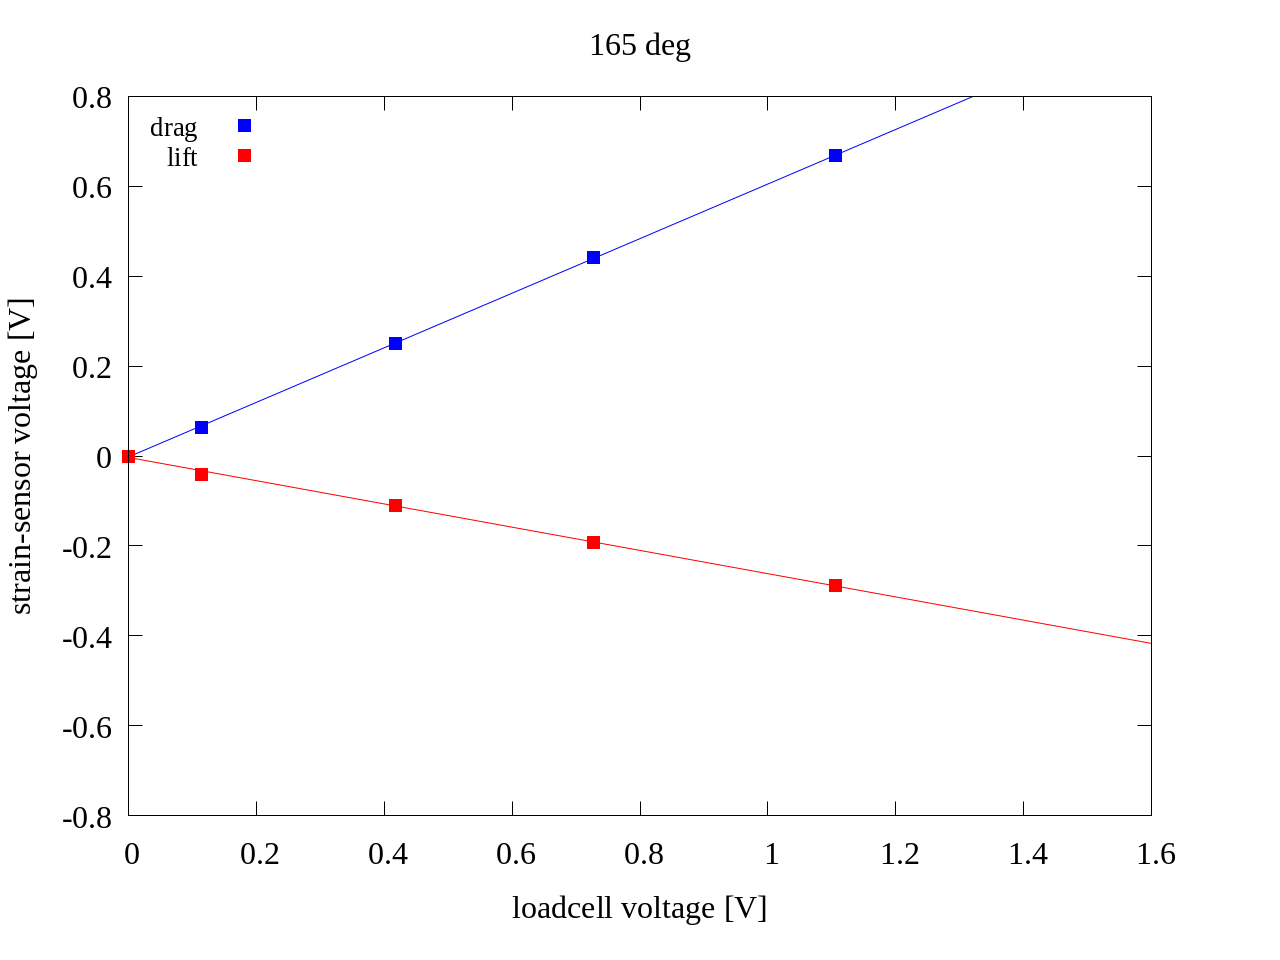
\includegraphics[width=78mm]{../images/linear/165_linear.png}
        \caption{Result of 165 deg}
    \end{center}
\end{figure}

\par
\newpage

\begin{figure}[htbp]
    \footnotesize
    \begin{center}
        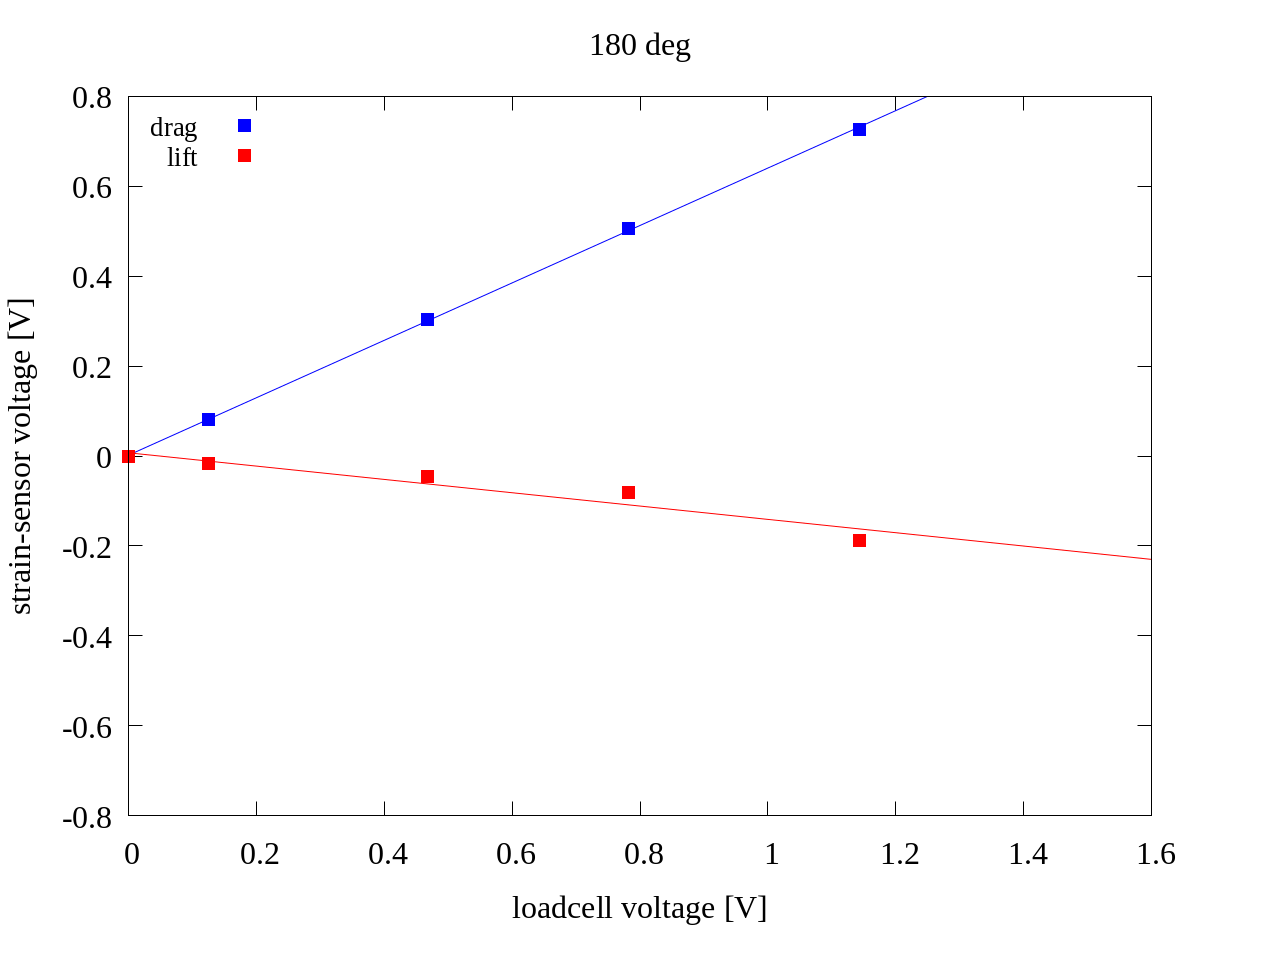
\includegraphics[width=78mm]{../images/linear/180_linear.png}
        \caption{Result of 180 deg}
        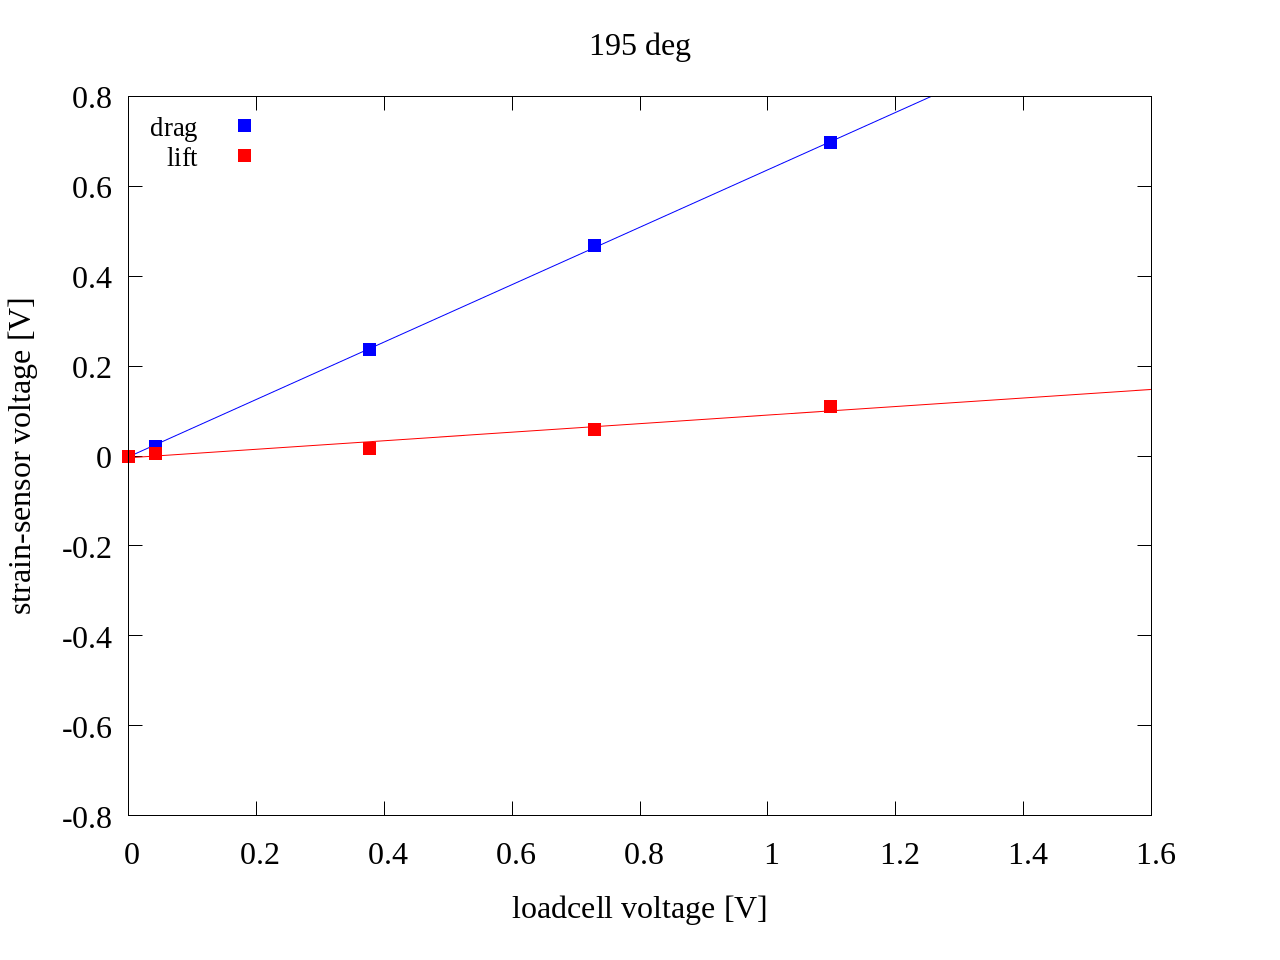
\includegraphics[width=78mm]{../images/linear/195_linear.png}
        \caption{Result of 195 deg}
        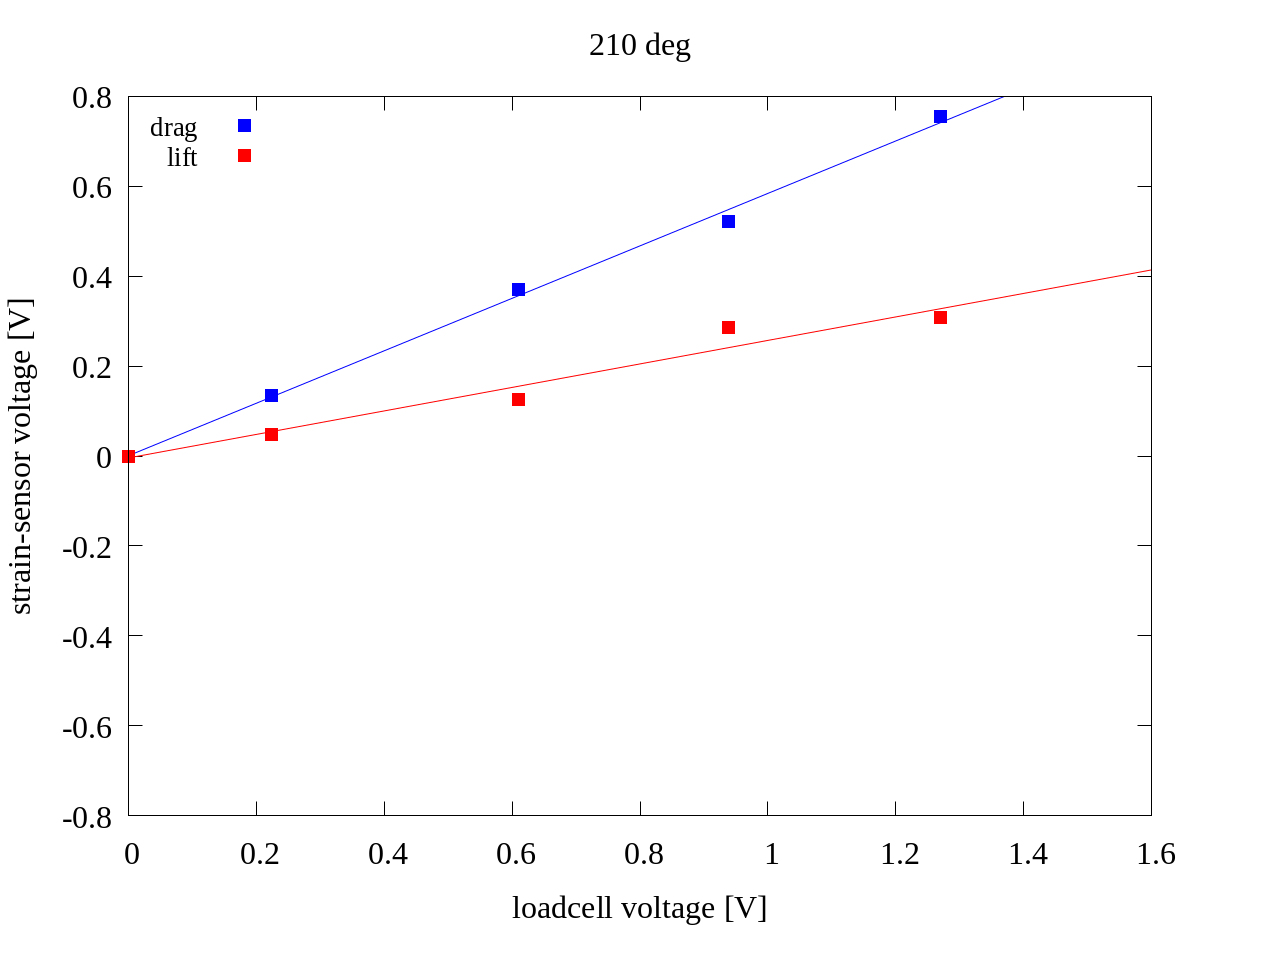
\includegraphics[width=78mm]{../images/linear/210_linear.png}
        \caption{Result of 210 deg}
        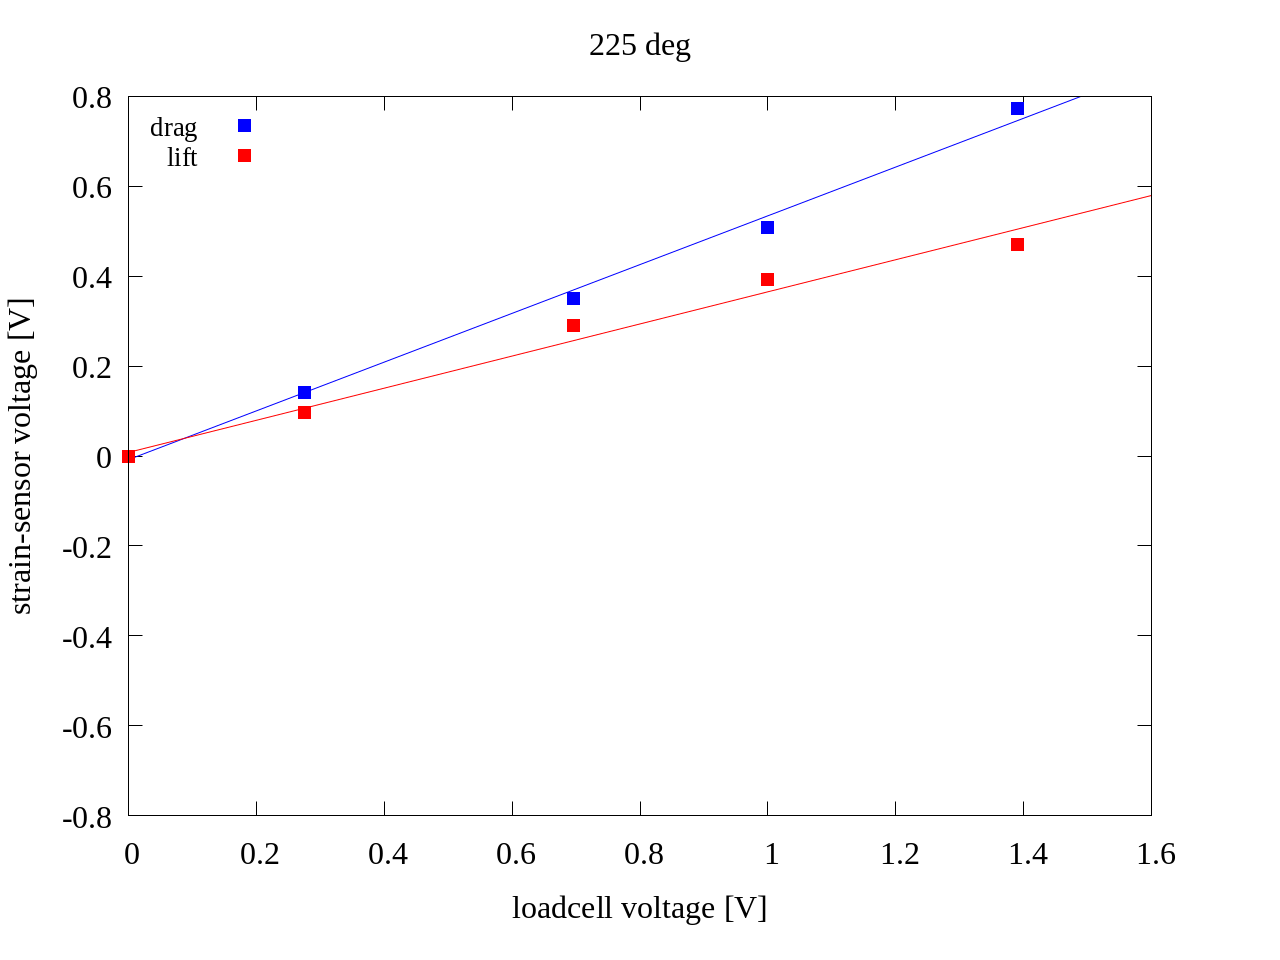
\includegraphics[width=78mm]{../images/linear/225_linear.png}
        \caption{Result of 225 deg}
    \end{center}
\end{figure}

\begin{figure}[htbp]
    \footnotesize
    \begin{center}
        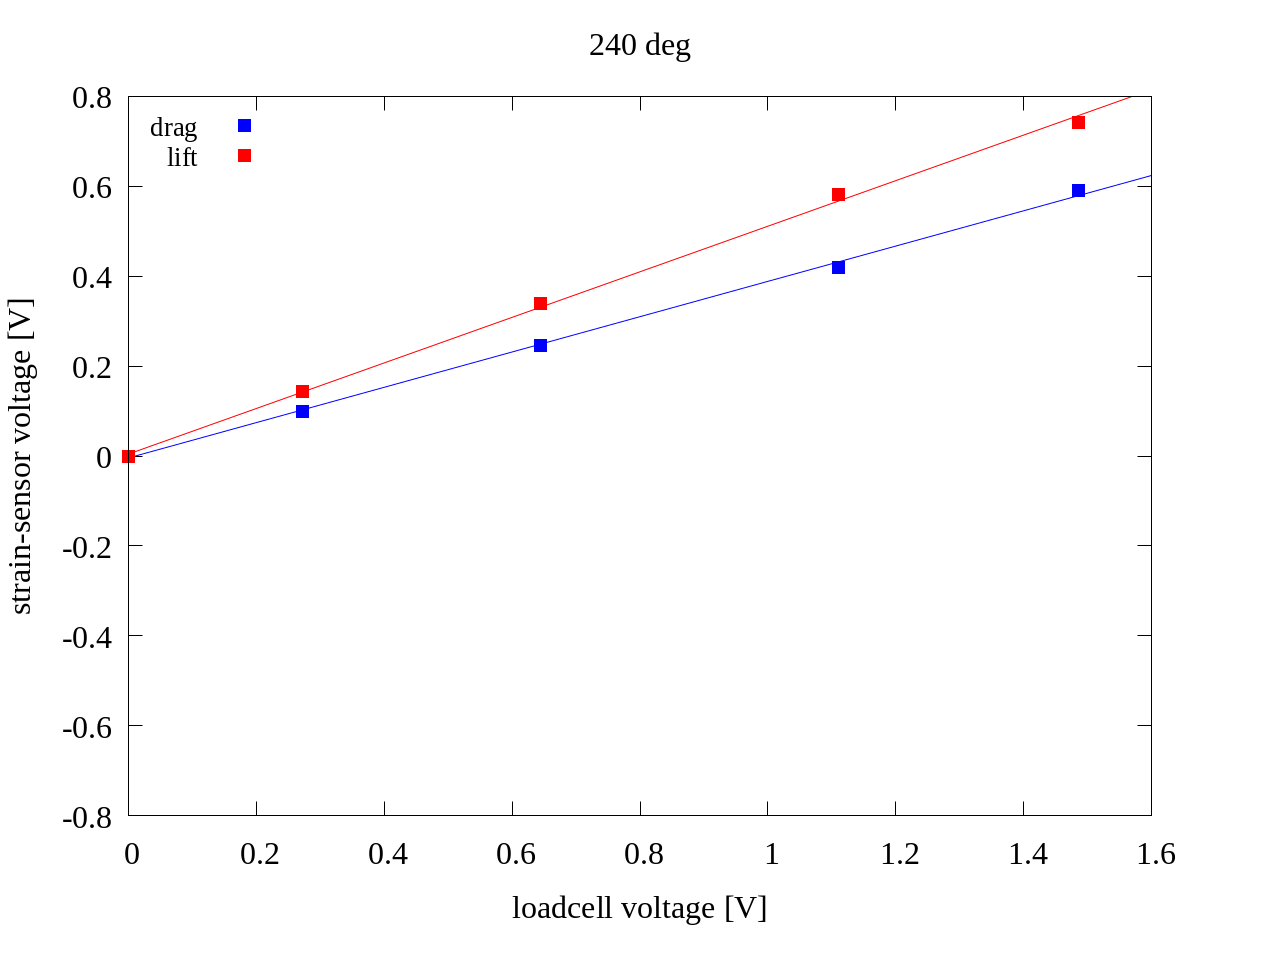
\includegraphics[width=78mm]{../images/linear/240_linear.png}
        \caption{Result of 240 deg}
        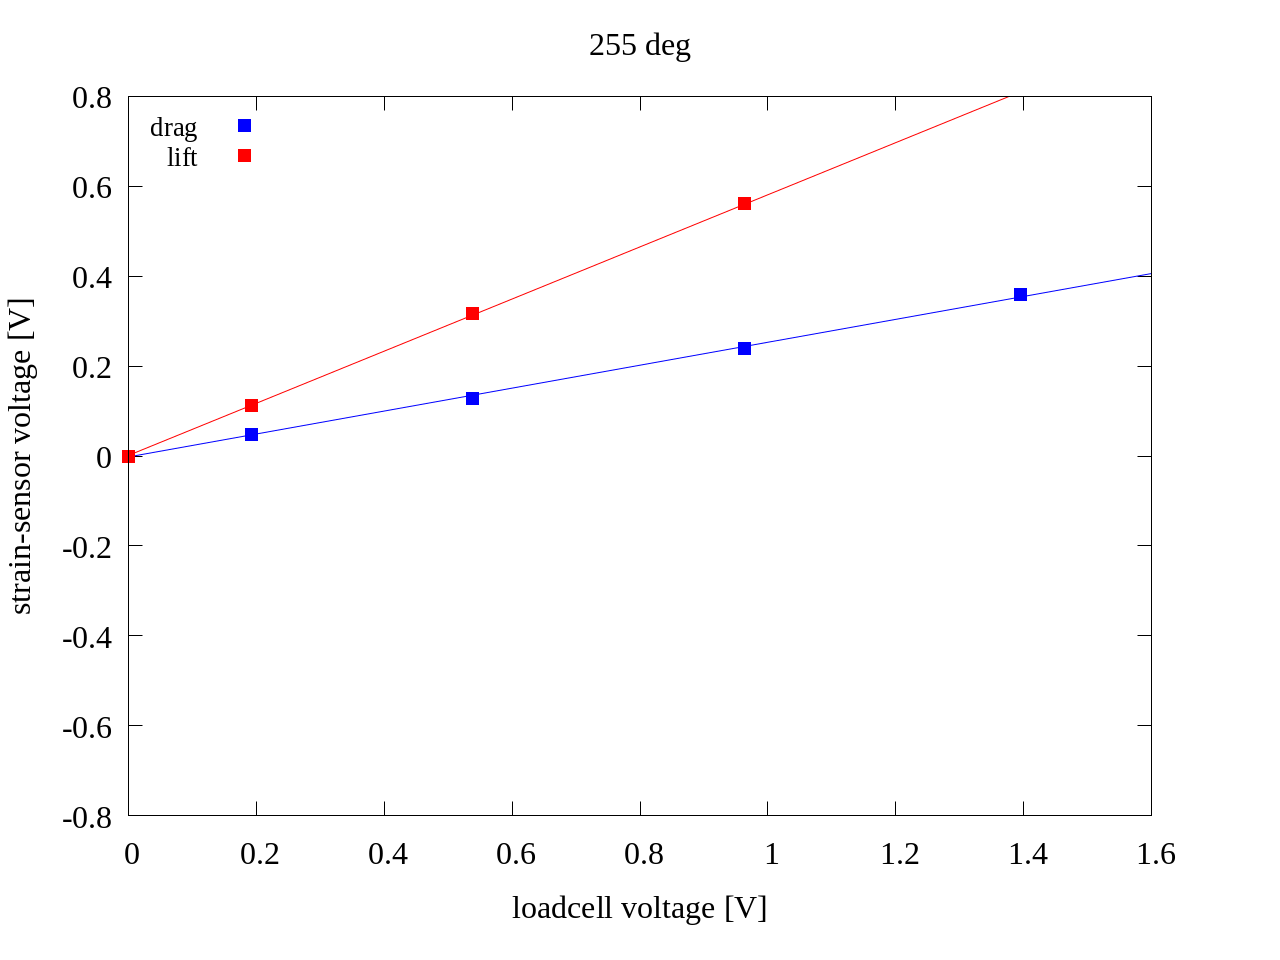
\includegraphics[width=78mm]{../images/linear/255_linear.png}
        \caption{Result of 255 deg}
        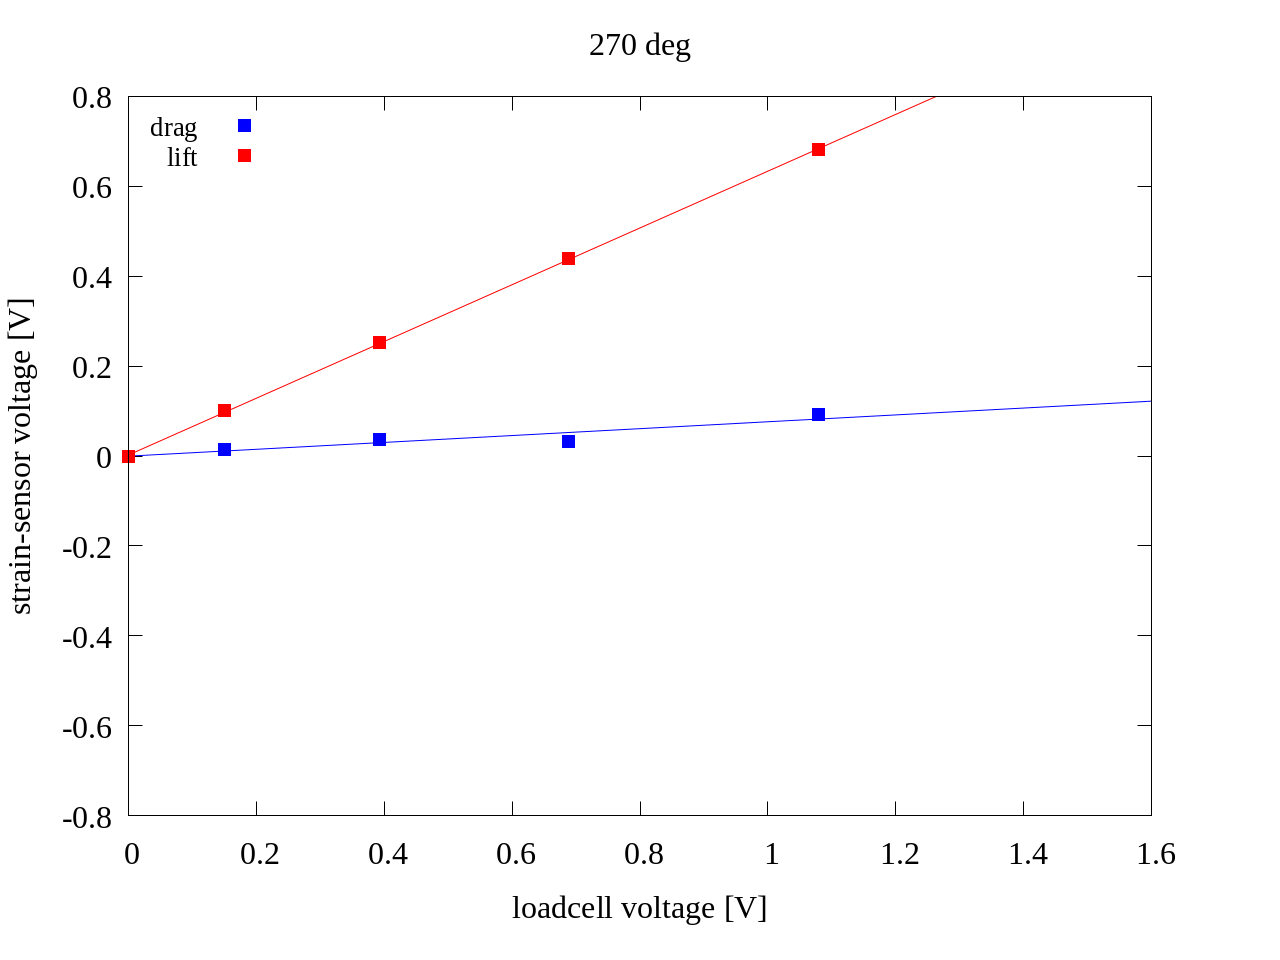
\includegraphics[width=78mm]{../images/linear/270_linear.png}
        \caption{Result of 270 deg}
        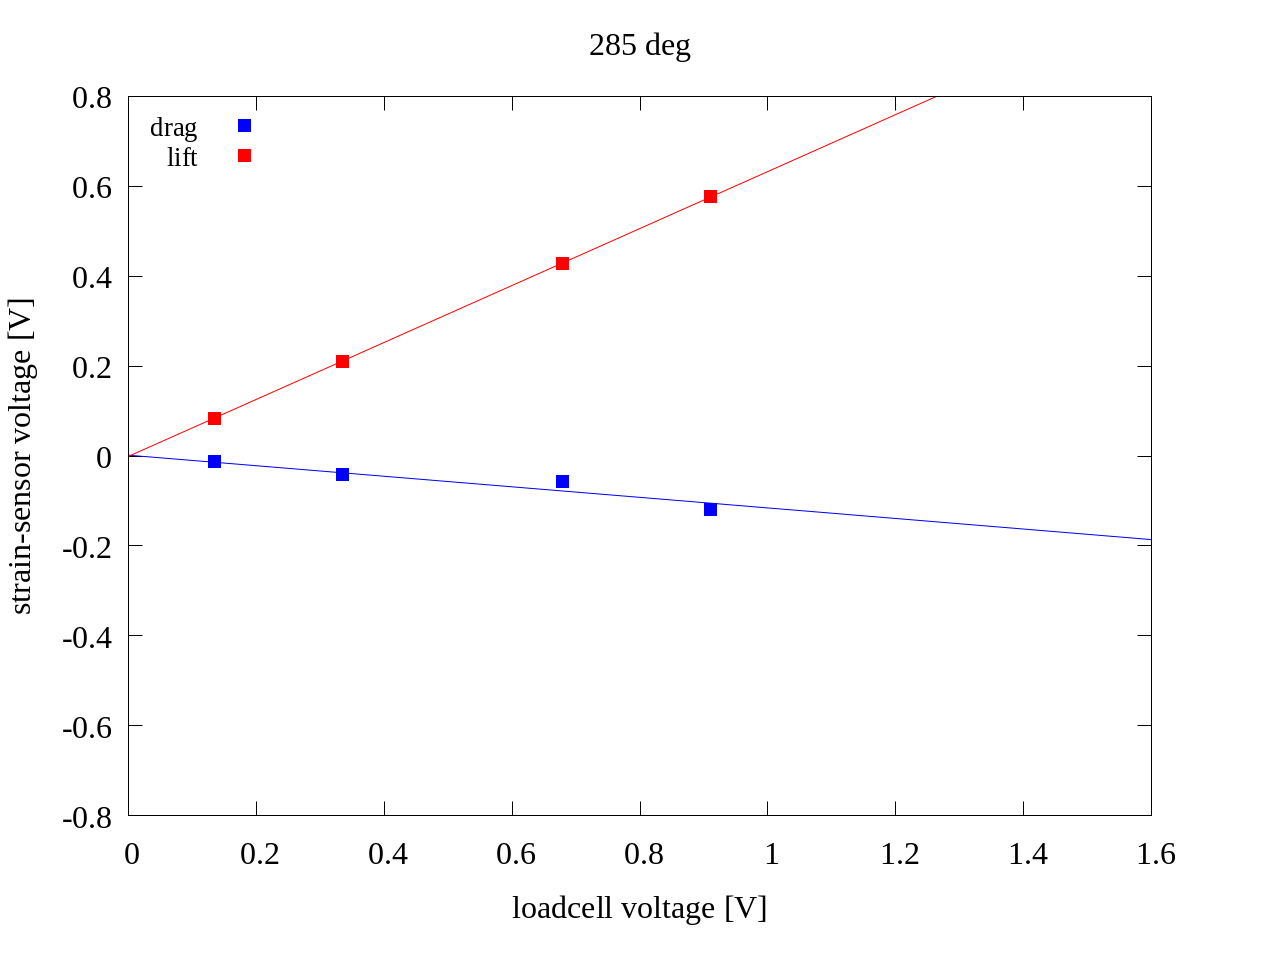
\includegraphics[width=78mm]{../images/linear/285_linear.png}
        \caption{Result of 285 deg}
    \end{center}
\end{figure}

\begin{figure}[htbp]
    \footnotesize
    \begin{center}
        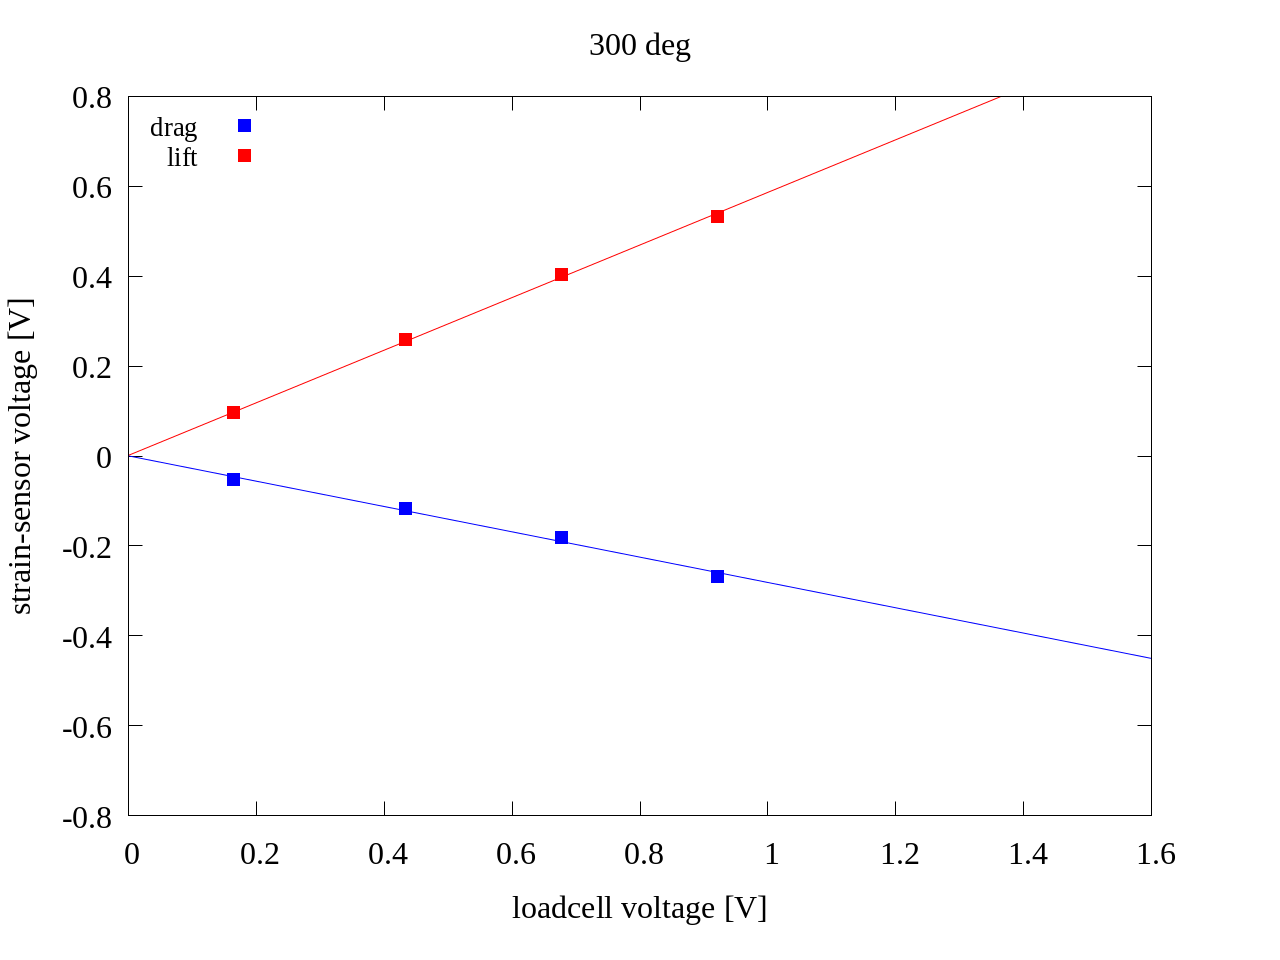
\includegraphics[width=78mm]{../images/linear/300_linear.png}
        \caption{Result of 300 deg}
        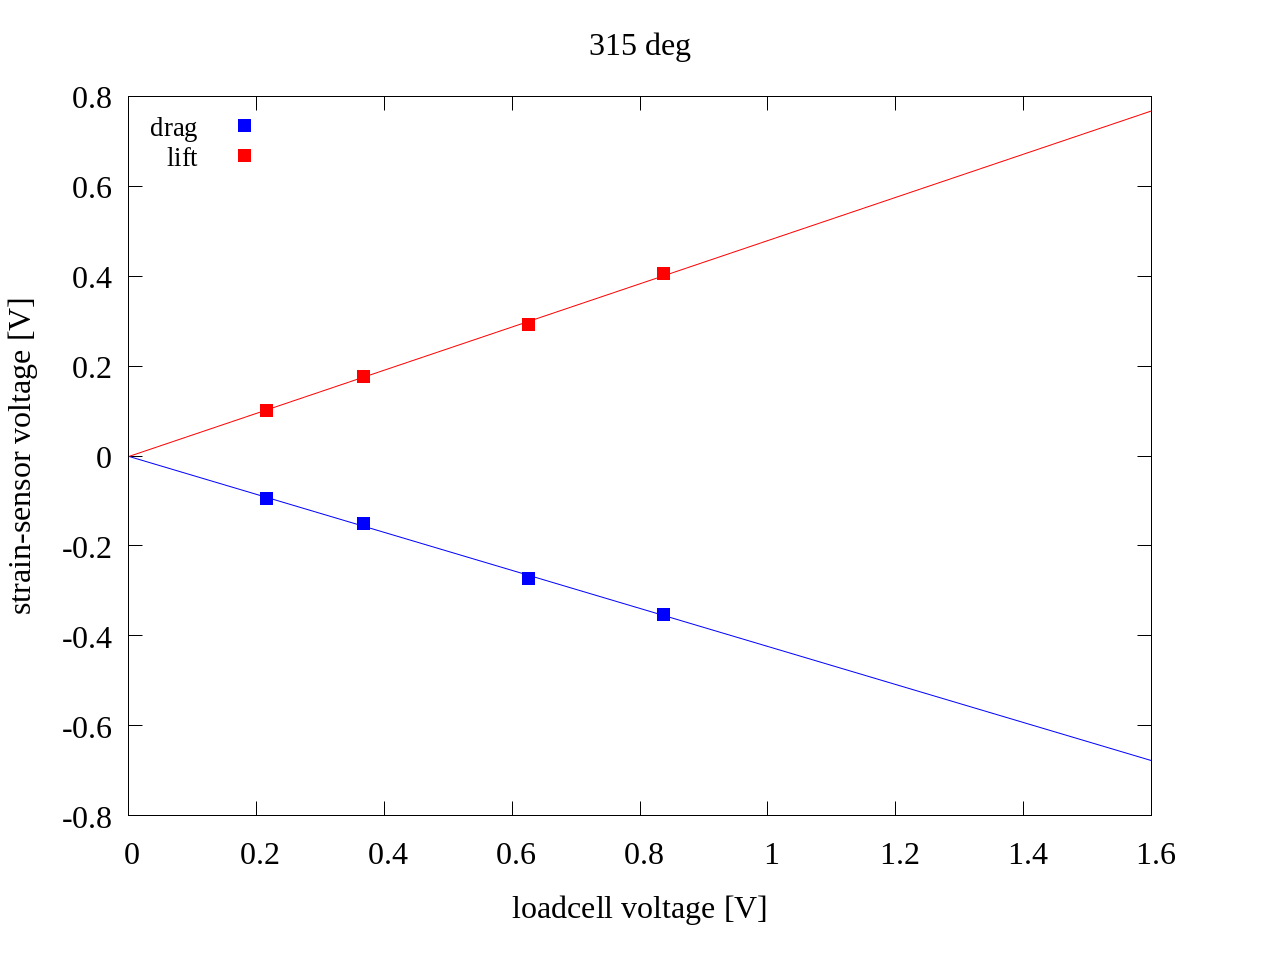
\includegraphics[width=78mm]{../images/linear/315_linear.png}
        \caption{Result of 315 deg}
        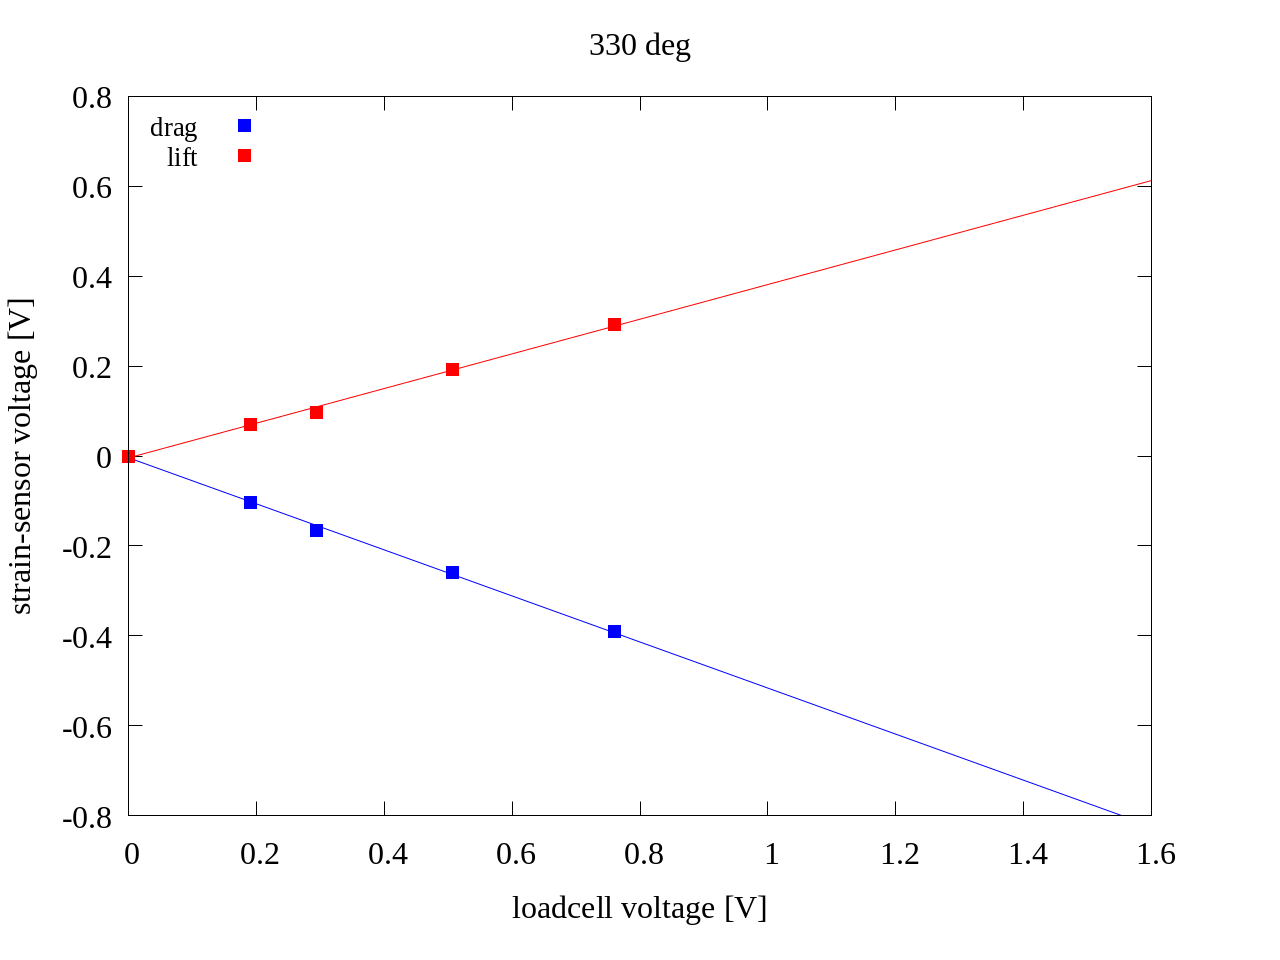
\includegraphics[width=78mm]{../images/linear/330_linear.png}
        \caption{Result of 330 deg}
        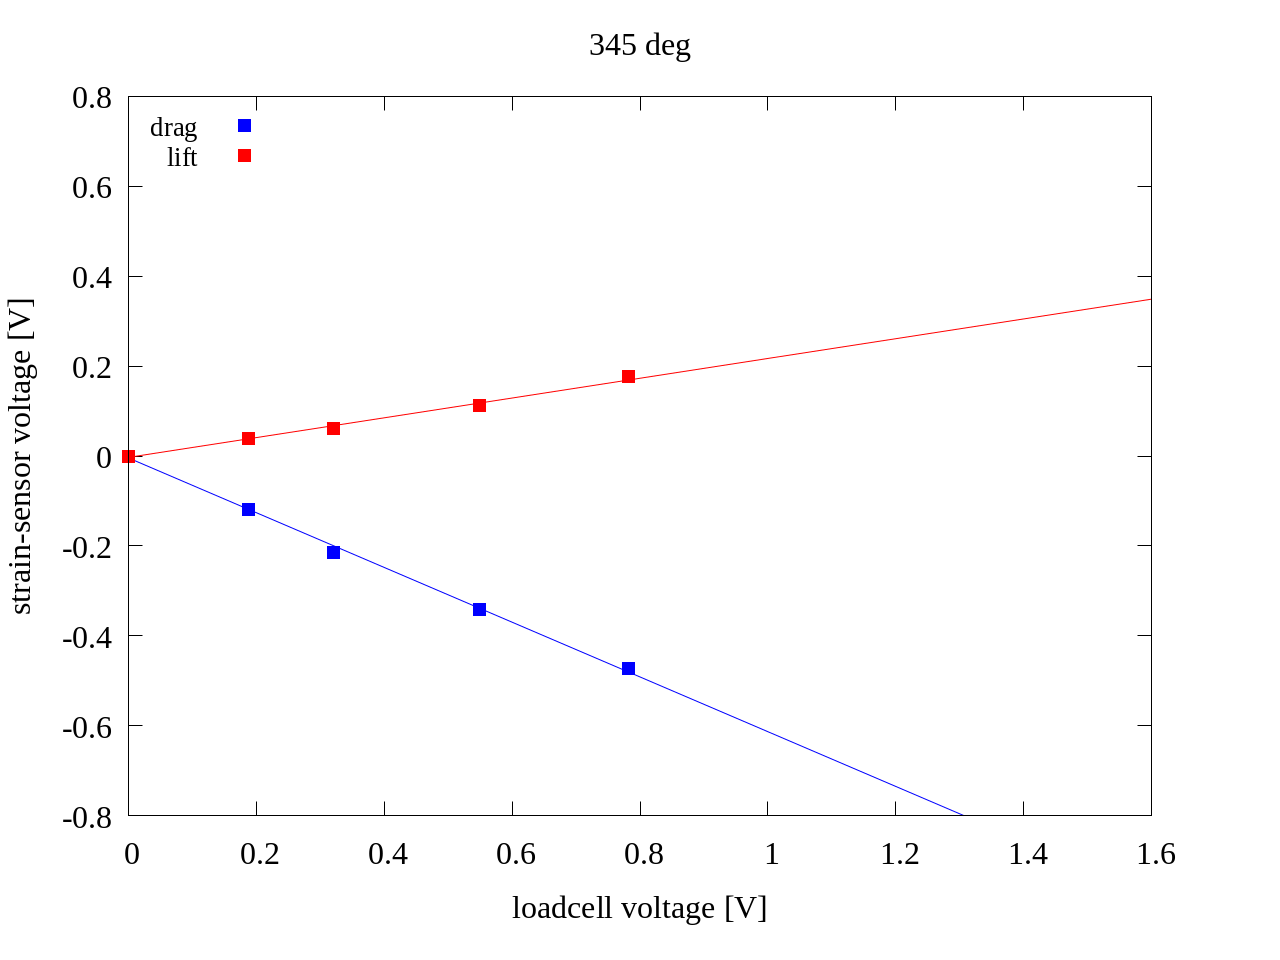
\includegraphics[width=78mm]{../images/linear/345_linear.png}
        \caption{Result of 345 deg}
    \end{center}
\end{figure}

\end{document}